
\section{State of the art}

\begin{itemize}
    \item ECAI23: \cite{HuangMS23} Given a DT computing a total classification function, creates a DS with: (1) No default rule, (2) No overlap, (3) total classification, and (4) each rule is a path AXp of the original DT.
Code available in \url{https://github.com/xuanxiangHuang/dtree2dset}

The main algorithm in the paper is shown in Algorithm~\ref{alg:DT2DS}.
For every path in the DT, it computes its AXp and creates a rule for the DS (line~7).

\begin{algorithm}
    \caption{Converting DT to DS}
    \label{alg:DT2DS}
    
    \KwIn{Decision Tree $\mathcal{T}$ with classification function $\kappa$}
    \KwOut{Decision Set $\mathcal{S}$}
    
    $\mathcal{S} \leftarrow \emptyset$\;
    $\mathbb{P} \leftarrow \text{AllPaths}(\mathcal{T})$\;
    \While{$P \neq \emptyset$}{
        $\mathcal{P}_k \leftarrow \text{PickPath}(\mathcal{P})$ \;
        \tcp*[r]{$\mathcal{P}_k$: some path not yet explained} 
        $\mathbb{P} \leftarrow \mathbb{P} \setminus \{\mathcal{P}_k\}$\;
        $\mathcal{X} \leftarrow \text{FindPathAXp}(\mathcal{P}_k)$\;
        $\mathcal{S} \leftarrow \mathcal{S} \cup 
        \{\text{IF } \bigwedge_{A \in \Lambda(\mathcal{P}_k)} l \text{ THEN } \kappa(\cdot) = c\}$\;
    }
    $\mathcal{S} \leftarrow \text{RemoveDuplicateRules}(\mathcal{S})$\;
    \Return{$S$}
\end{algorithm}

    \item JAIR22: \cite{izza-jair-22} Redundancies in Path Explanations for DT. In Section~5, Abductive Path Explanation by: (5.1) Explicit path analysis, (5.2) Tree Traversal, (5.3) Horn Encoding.
(5.4) Contrastive Path Explanation.
(5.5) Enumeration of Path Explanations.

The main algorithm from Section 5.2 is in Algorithm~\ref{alg:FindAXp}.
It iteratively removes features from the AXp, checking if it exsits a consistent path.
This checking is performed in Algorithm~\ref{alg:ExistsConsistentQPath}.
Recursively, it traverses the tree, checking if it exists a consistent path.

\begin{algorithm}
\caption{Computing one path explanation (or path-restricted AXp)}
\label{alg:FindAXp}

\KwIn{Decision Tree $\mathcal{T}$, Features $\mathcal{F}$, Path $P_k$}
\KwOut{Path-restricted AXp}

$U \leftarrow \mathcal{F} \setminus P_k$
\tcp*[r]{Features $\notin$ path also $\notin$ APXp}
\For{$i \in \Phi(P_k)$}{
    $\mathcal{U} \leftarrow \mathcal{U} \cup \{i\}$ 
    \tcp*[r]{Tentatively drop $i$ from APXp}
    \If{$\text{ExistsConsistentQPath}(P_k, \mathcal{U}, \text{root}(\mathcal{T}))$}{
        $\mathcal{U} \leftarrow \mathcal{U} \setminus \{i\}$
        \tcp*[r]{Feature $i$ must be included in APXp}
    }
}
\Return{$\mathcal{F} \setminus \mathcal{U}$} \tcp*{Return APXp}
\end{algorithm}

\begin{algorithm}
\caption{Checking consistent path to prediction in $\mathcal{K} \setminus \{c\}$}
\label{alg:ExistsConsistentQPath}

\KwIn{Path $P_k$, Features $\mathcal{U}$, Node $r$}

\If{$r$ is terminal}{
    \If{$\zeta(r) \neq \zeta(\tau(P_k))$}{
        \Return{true} \tcp*[r]{Found consistent path to $d \neq c$}
    }
    \Else{
        \Return{false} \tcp*[r]{Not a consistent path to $d \neq c$}
    }
}
$i \leftarrow \phi(r)$ \tcp*[r]{Pick feature associated with node $r$}
\For{$s \in \sigma(r)$}{
    \tcp*[r]{Recursively traverse child nodes, as long as}
    \tcp*[r]{edge values exhibit consistent values}
    \If{$(i \in \mathcal{U}) \lor (\rho(i, P_k) \cap \epsilon((r, s)) \neq \emptyset)$}{
        \If{$\text{ExistsConsistentQPath}(P_k, \mathcal{U}, s)$ }{
            \Return{true} \tcp*[r]{ Found consistent path to $d \neq c$}
        }
    }
}
\Return{false} \tcp*[r]{ Unable to find consistent path to $d \neq c$}
\end{algorithm}

The \emph{hpath-unrestricted} Horn encoding in Section 5.3 is the following:

\begin{description}
    \item[H1] For the root node $\top \rightarrow b_r$.
    \item[H2] For each terminal node with prediction $c$ add the constraint $\top \rightarrow b_r$.
    \item[H3] For each internal node with prediction $\neq c$ add the constraint $a_i \rightarrow b_i$.
    \item[H4] For a node $r$ associated with feature $i$ and connected to 
    the child $s$ \emph{consistent} with the value of $i$ in $v$, add the constraint
    $b_r \rightarrow b_s$.
    \item[H5] For a node $r$ associated with feature $i$ and connected to 
    the child $s$ \emph{inconsistent} with the value of $i$ in $v$, add the constraint
    $b_r \land u_i \rightarrow b_s$.
\end{description}

\begin{example}

    Given the instance $(\mathbf{v} = \{1\}, c=1)$ and the short example in Figure~\ref{fig:horn-dt}, the Horn encoding is
    the following hard clauses:
    \begin{align*}
        \top &\rightarrow b_0 \\
        b_0 &\rightarrow b_1 \\
        b_0 &\land u_1 \rightarrow b_2
    \end{align*}
    (where $u_1$ corresponds to universal $v_1$), and the following soft clauses:
    \begin{align*}
        u_1
    \end{align*}

    \begin{figure}
        \centering
        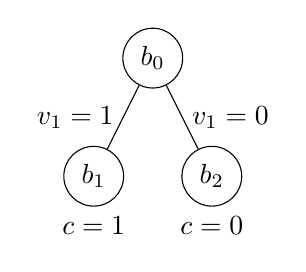
\begin{tikzpicture}
            \node[circle, draw] (root) {$b_0$}
                child {node[circle, draw, label=below:{$c=1$}] {$b_1$} edge from parent node[left] {$v_1=1$}}
                child {node[circle, draw, label=below:{$c=0$}] {$b_2$} edge from parent node[right] {$v_1=0$}};
        \end{tikzpicture}
        \caption{Example of the Horn encoding for a decision tree}
        \label{fig:horn-dt}
    \end{figure}

\end{example}

\item AAAI24: \cite{IzzaISM24}. It computes inflatex abductive explanations.
%
Inflated explanations is a set of features and for each feature a set of values 
such that the decision will remain unchanged, for any of the values allowed
for any of the features in the (inflated) abductive explanation.
%
Tha main algorithm is shown in Algorithm~\ref{alg:InflateAXp}.

\begin{algorithm}
\caption{Computing inflated explanations}
\label{alg:InflateAXp}

\KwIn{$\mathcal{E} = (M, (v, c)), AXp X \subseteq F, Precision\ \delta$}
\KwOut{X, X}

{InflateAXp}{E, X}
    $X \gets \emptyset$ \tcp*[r]{X: Sets composing inflated explanation}
    $\iota \gets PickSomeOrder(X')$\;
    \For{$j \in \iota$} {
        \If{Categorical(j)} {
            $\mathbb{E}_j \gets \{v_j\}$ \;
            $\mathbb{E}_j \gets InflateCategorical(j, \mathbb{E}_j, \mathcal{E}, X')$ \;
        } \Else {
            $inf(j) \gets sup(j) \gets v_j$\; 
            $\mathbb{E}_j \gets [inf(j), sup(j)]$\; \tcp*[r]{Initial $\mathbb{E}_j$}
            $\mathbb{E}_j \gets InflateOrdinal(j, \mathbb{E}_j, \mathcal{E}, X', \delta)$\;
        }
        $X \gets X \cup \{(j, \mathbb{E}_j)\}$
    }
    \Return{X, X}
\end{algorithm}

\item SAT21: \cite{IgnatievS21} Section 3.2. Explaining Arbitrary DLs with SAT.
In this section the following constraint is defined:

Let \(\mathbf{v}\) denote a point in feature space with prediction \(c \in \mathcal{K}\). Moreover, let the rule that fires on \(\mathbf{v}\) be \(i \in \mathcal{R}\). Note that for an arbitrary rule \(k \in \mathcal{R}\) to fire, the following constraint must hold true:
\[
\bigwedge_{r_j \in \mathcal{R} \atop o(j) < o(k)} \neg(l(j)) \land l(k)
\]

This constraint encodes the fact that the literals in all the rules preceding rule
$k$ must not fire and the rule $k$ must fire. (Recall that $l(i)$ represents the set of
literals of rule $i$). 

\item IJCAI23: \cite{Audemard23}
It encodes the problem of finding a minimal abductive explanation for a boosted 
regression tree as a MILP problem.

Every term $t$ over $\mathcal{B}$ that is consistent (i.e., $t$ does not
contain both an element of $\mathcal{B}$ and its negation) can be \emph{simplified} 
using $\Sigma$. Thus, each time $t$ contains two distinct literals $\ell$ and 
$\ell'$ such that $\ell'$ is entailed by $\ell$ given $\Sigma$, $\ell'$
can be removed from $t$. The specific nature of $\Sigma$ ensures that such a 
simplification process is \emph{confluent}, i.e., the term obtained at the end of the 
simplification process (called the \emph{simplification of} $t$ \emph{given} 
$\Sigma$ ) is uniquely defined whatever the ordering according to which the literals are 
considered (this would not be ensured if $\Sigma$ was any formula over $\mathcal{B}$). 
Thus, when simplified, $t$ cannot contain more than one positive (resp. negative) 
literal issued from the same numerical attribute $A_i$ and more than one positive 
literal issued from the same categorical attribute $A_i$ (and if such a positive 
literal exists, $t$ does not contain any negative literal issued from $A_i$). 
By construction, the simplification of $t$  given $\Sigma$ is equivalent to $t$
under $\Sigma$. Furthermore, the simplification of $t$ given $\Sigma$ can be 
computed in time $\mathcal{O}(|\Sigma| \cdot |t|^2)$.


\end{itemize}


\subsection{Enumeration of Explanation}

The enumeration of AXp and CXp can be done with the algorithm in~\cite{MSGCIN20}
and with algorithm Marco~\cite{LiffitonM13}, shown in Algorithm~\ref{alg:marco}.

\begin{algorithm}
    \caption{MARCO algorithm}\label{alg:marco}
    \KwIn{Unsatisfiable constraint set \( C = \{C_1, C_2, C_3, \dots, C_n\} \)}
    \KwOut{MSSes and MUSes of \( C \) as they are discovered}
    $Map \gets \text{BoolFormula}(nvars = |C|)$ \tcp*[r]{Empty formula over $|C|$ Boolean variables}
    \While{$Map$ is satisfiable}{
        $m \gets \text{getModel}(Map)$\;
        $seed \gets \{C_i \in C : m[x_i] = \text{True}\}$ \tcp*[r]{Project the assignment $m$ onto $C$}
        \eIf{$seed$ is satisfiable}{
            $MSS \gets \text{grow}(seed, C)$\;
            \KwYield $MSS$\;
            $Map \gets Map \land \text{blockDown}(MSS)$\;
        }{
            $MUS \gets \text{shrink}(seed, C)$\;
            \KwYield $MUS$\;
            $Map \gets Map \land \text{blockUp}(MUS)$\;
        }
    }
\end{algorithm}

The application of Marco algorithm to enumeration of AXp's and CXp's was 
explained in~\cite{IgnatievNA020}.
There are also algorithms for particular cases, monotonic classifiers~\cite{MarquesSilvaGCIN21} and decision lists~\cite{IgnatievS21}.

We can see how the algorithm works with the following example.

\begin{example}
    Given a set of features $\mathcal{A} = \{x_1, x_2, x_3\}$.
    %
    Let a formula be
    $\phi = (x_1 \land x_2) \lor (x_2 \land x_3)$, 
    and an instance $\mathbf{x} = \{1, 1, 1\}$.
    It's straightforward to see 
    that its AXp's and CXp's are:
    \begin{eqnarray*}
    AXp's &:& \{ 1, 2 \}, \{ 2, 3 \} \\
    CXp's &:& \{1, 3\}, \{2\}
    \end{eqnarray*}

    In  Figure~\ref{fig:lattice1}, the circles correspond to the AXp's, 
    and to the rest of node correspond to the WCXp's. 
    %
    A set in a node represents the set of literals for an WAXP, 
    and the complementary set of literals for a WCXP.
    %
    The AXp's are the minimal points of the set of WAXp's, 
    and the CXp's are the maximal points of the set of WCXp's,
    being the lattice subset-minimal ordered.
    These sets are plotted in the lattice in gray.

    \begin{figure}
        \begin{center}
        
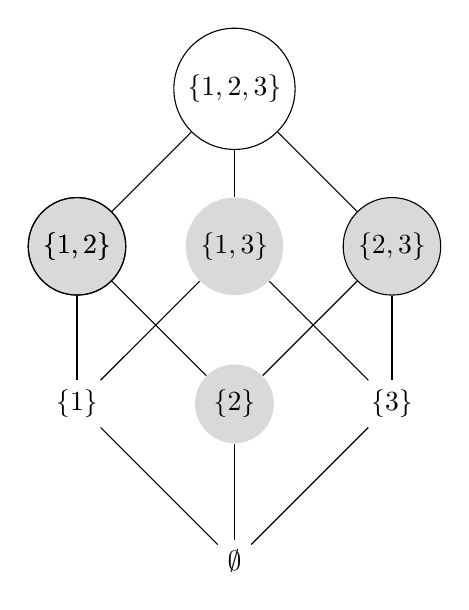
\begin{tikzpicture}%[scale=1.5, transform shape, every node/.style={draw, circle, minimum size=1cm}]
    % Define the subsets
    \node (empty) at (0,0) {$\emptyset$};
    \node (1) at (-2,2) {$\{1\}$};
    \node[circle, minimum size=1cm, fill=gray!30] (2) at (0,2) {$\{2\}$};
    \node (3) at (2,2) {$\{3\}$};
    \node[draw, circle, minimum size=1cm, fill=gray!30] (12) at (-2,4) {$\{1, 2\}$};
    \node[circle, minimum size=1cm, fill=gray!30] (13) at (0,4) {$\{1, 3\}$};
    \node[draw, circle, minimum size=1cm, fill=gray!30] (23) at (2,4) {$\{2, 3\}$};
    \node[draw, circle, minimum size=1cm] (123) at (0,6) {$\{1, 2, 3\}$};
    
    \node[draw, circle, minimum size=1cm] (12) at (-2,4) {$\{1, 2\}$};

    % Draw the edges
    \draw (empty) -- (1);
    \draw (empty) -- (2);
    \draw (empty) -- (3);
    \draw (1) -- (12);
    \draw (1) -- (13);
    \draw (2) -- (12);
    \draw (2) -- (23);
    \draw (3) -- (13);
    \draw (3) -- (23);
    \draw (12) -- (123);
    \draw (13) -- (123);
    \draw (23) -- (123);
\end{tikzpicture}


        \end{center}
    \caption{Lattice for the example.}\label{fig:lattice1}
    \end{figure}

\end{example}

